% !TEX encoding = UTF-8 Unicode
% !TEX spellcheck = en_US

\subsection{Experiment Scenario}
\label{subsec:ExperimentScenario}

As described in Sec.\,\ref{subsec:Introduction}, a parameter identification in the process environment is rarely feasible without restrictions regarding the available workspace. For this reason, the approach of the method presented in this paper is based on performing the necessary parameter identification directly in the running process. To illustrate this situation, the proposed method is applied to two different tasks widely used in industry. These processes are presented in more detail in the following paragraph. 
\begin{itemize}
\item Process 1: The robot performs a highly dynamic \textit{pick and place} motion between two pre-defined areas in the workspace (see Fig.\,\ref{fig:Process1}.a). To create a set of \textit{pick-and-place} cycles the points on both areas are generated randomly.
\item Process 2: The end-effector of the robot has to trace the edges of a horizontal square (see Fig.\,\ref{fig:Process1}.b).
\end{itemize}
To validate the identified parameters, different trajectories of the same type are used for each process. For process 1 a new set of points is randomly generated using a uniform distribution. For process 2 the trajectory is given an offset in the $x$-$y$-plane.

%\begin{figure*}[tb]
%  \vspace{-0.2cm}
%  \centering
%   \includegraphics[width = 18cm]{Chapters/Experiments/Experimental_Design/SzenarienKompakt.pdf}
%  \caption{Representation of process 1 and 2 and the restricted robot workspace.}
%  \label{fig:Process1}
%  \vspace{-0.1cm}
%\end{figure*}

%\begin{figure}[tb]
%  \vspace{-0.2cm}
%  \centering
%   \includegraphics[width = 7.5cm]{Chapters/Experiments/Experimental_Design/Szenario_PnP.pdf}
%  \caption{Representation of process 1 in the robot workspace.}
%  \label{fig:Process1}
%  \vspace{-0.1cm}
%\end{figure}

%\begin{figure}[tb]
%  \vspace{-0.2cm}
%  \centering
%   \includegraphics[width = 7.5cm]{Chapters/Experiments/Experimental_Design/Szenario_Square.pdf}
%  \caption{Representation of process 2 in the robot workspace.}
%  \label{fig:Process2}
%  \vspace{-0.1cm}
%\end{figure}

To evaluate the results of the process-based parameter identification a classical parameter identification with three different optimized excitation trajectories is also carried out. The first excitation trajectory uses the full workspace of the robot to get the best possible identification results. For the second trajectory the available robot workspace is restrained to simulate the identification process under practical conditions in the industrial environment. A representation of the used workspace is given in Fig.\,\ref{fig:Process1}.c. The complete half-sphere represents the full workspace. The marked area denotes the restrained workspace. The optimized excitation trajectories are generated according to Sec.\,\ref{subsec:OptimalExcitation}. The trajectory which uses the full workspace has a condition number of 6.76 and will be called \textit{trajectory A}. The trajectory in the restrained workspace has a condition number of 7.71 and will be called \textit{trajectory B}. Restraining the available workspace generally leads to higher condition numbers of the generated excitation trajectory. The third trajectory is used to validate both models derived from the optimal excitation and will be called \textit{trajectory C}. Like \textit{trajectory A}, \textit{trajectory C} is generated in the full workspace of the robot but uses a different set of \textsc{Fourier}-coefficients, due to the heuristic nature of the genetic algorithm. The identification was performed without model-based feedforward control.

%\begin{figure}[tb]
%  \vspace{-0.2cm}
%  \centering
%   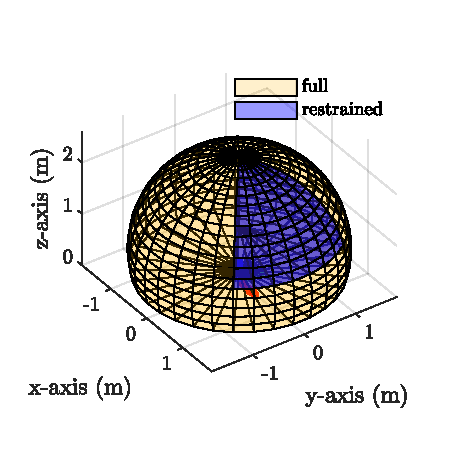
\includegraphics[width = 7.5cm]{Chapters/Experiments/Experimental_Design/TaskSpace.pdf}
%  \caption{Representation of the used workspace during optimized excitation.}
%  \label{fig:TaskSpace}
%  \vspace{-0.1cm}
%\end{figure}


%\begin{figure*}[tb]
%   \centering
%   \begin{subfigure}{0.3\textwidth}
%        %\vspace{-0.2cm}
%        \centering
%            \includegraphics[width = \textwidth]{Chapters/Experiments/Experimental_Design/Szenario_PnP.pdf}
%        \caption{Representation of process 1 in the robot workspace.}
%        \label{fig:Process1}
%        %\vspace{-0.1cm}
%    \end{subfigure}%
%    
%    \begin{subfigure}{0.3\textwidth}
%        %\vspace{-0.2cm}
%        \centering
%            \includegraphics[width = \textwidth]{Chapters/Experiments/Experimental_Design/Szenario_Square.pdf}
%        \caption{Representation of process 2 in the robot workspace.}
%        \label{fig:Process2}
%        %\vspace{-0.1cm}
%    \end{subfigure}%
%    
%    \begin{subfigure}{0.3\textwidth}
%        %\vspace{-0.2cm}
%        \centering
%            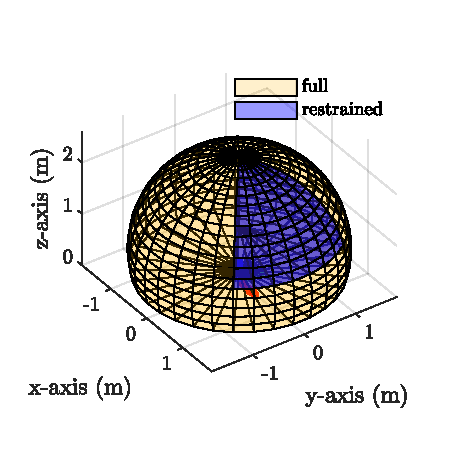
\includegraphics[width = \textwidth]{Chapters/Experiments/Experimental_Design/TaskSpace.pdf}
%        \caption{Representation of the used workspace during optimized excitation.}
%       \label{fig:TaskSpace}
%        %\vspace{-0.1cm}
%    \end{subfigure}%
%    \caption{Representation of process 1 and 2 and the restricted robot workspace.}
%\end{figure*}

\begin{figure*}[tb]
  \vspace{-0.2cm}
  \centering
    %\subfigure[Representation of process 1 in the robot workspace.]{\includegraphics[width = 5.5cm]{Chapters/Experiments/Experimental_Design/Szenario_PnP.pdf}}
    %\subfigure[Representation of process 2 in the robot workspace.]{\includegraphics[width = 5.5cm]{Chapters/Experiments/Experimental_Design/Szenario_Square.pdf}}
    %\subfigure[Representation of the used workspace during optimized excitation.]{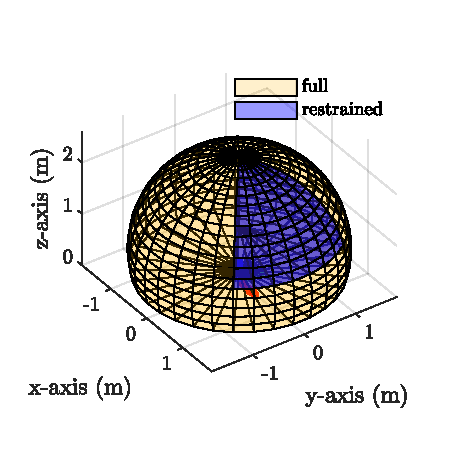
\includegraphics[width = 5.5cm]{Chapters/Experiments/Experimental_Design/TaskSpace.pdf}}
    \includegraphics{Chapters/Experiments/Experiment_Scenario/SzenarienKompakt.pdf}
  \vspace{-0.2cm}
  \caption{Representation of process 1 and 2 and the workspace used for optimization.}
  \label{fig:Process1}
  \vspace{-0.3cm}
\end{figure*}